\documentclass[a4paper,
fontsize=11pt,
%headings=small,
oneside,
numbers=noperiodatend,
parskip=half-,
bibliography=totoc,
final
]{scrartcl}

\usepackage[babel]{csquotes}
\usepackage{synttree}
\usepackage{graphicx}
\setkeys{Gin}{width=.4\textwidth} %default pics size

\graphicspath{{./plots/}}
\usepackage[ngerman]{babel}
\usepackage[T1]{fontenc}
%\usepackage{amsmath}
\usepackage[utf8x]{inputenc}
\usepackage [hyphens]{url}
\usepackage{booktabs} 
\usepackage[left=2.4cm,right=2.4cm,top=2.3cm,bottom=2cm,includeheadfoot]{geometry}
\usepackage[labelformat=empty]{caption} % option 'labelformat=empty]' to surpress adding "Abbildung 1:" or "Figure 1" before each caption / use parameter '\captionsetup{labelformat=empty}' instead to change this for just one caption
\usepackage{eurosym}
\usepackage{multirow}
\usepackage[ngerman]{varioref}
\setcapindent{1em}
\renewcommand{\labelitemi}{--}
\usepackage{paralist}
\usepackage{pdfpages}
\usepackage{lscape}
\usepackage{float}
\usepackage{acronym}
\usepackage{eurosym}
\usepackage{longtable,lscape}
\usepackage{mathpazo}
\usepackage[normalem]{ulem} %emphasize weiterhin kursiv
\usepackage[flushmargin,ragged]{footmisc} % left align footnote
\usepackage{ccicons} 
\setcapindent{0pt} % no indentation in captions
\usepackage{xurl} % Breaks URLs

%%%% fancy LIBREAS URL color 
\usepackage{xcolor}
\definecolor{libreas}{RGB}{112,0,0}

\usepackage{listings}

\urlstyle{same}  % don't use monospace font for urls

\usepackage[fleqn]{amsmath}

%adjust fontsize for part

\usepackage{sectsty}
\partfont{\large}

%Das BibTeX-Zeichen mit \BibTeX setzen:
\def\symbol#1{\char #1\relax}
\def\bsl{{\tt\symbol{'134}}}
\def\BibTeX{{\rm B\kern-.05em{\sc i\kern-.025em b}\kern-.08em
    T\kern-.1667em\lower.7ex\hbox{E}\kern-.125emX}}

\usepackage{fancyhdr}
\fancyhf{}
\pagestyle{fancyplain}
\fancyhead[R]{\thepage}

% make sure bookmarks are created eventough sections are not numbered!
% uncommend if sections are numbered (bookmarks created by default)
\makeatletter
\renewcommand\@seccntformat[1]{}
\makeatother

% typo setup
\clubpenalty = 10000
\widowpenalty = 10000
\displaywidowpenalty = 10000

\usepackage{hyperxmp}
\usepackage[colorlinks, linkcolor=black,citecolor=black, urlcolor=libreas,
breaklinks= true,bookmarks=true,bookmarksopen=true]{hyperref}
\usepackage{breakurl}

%meta
%meta

\fancyhead[L]{Redaktion LIBREAS\\ %author
LIBREAS. Library Ideas, 47 (2025). % journal, issue, volume.
\href{https://doi.org/10.18452/x}{\color{black}https://doi.org/10.18452/x}
{}} % doi 
\fancyhead[R]{\thepage} %page number
\fancyfoot[L] {\ccLogo \ccAttribution\ \href{https://creativecommons.org/licenses/by/4.0/}{\color{black}Creative Commons BY 4.0}}  %licence
\fancyfoot[R] {ISSN: 1860-7950}

\title{\LARGE{Editorial \#47: Lug und Trug (im Wissenschaftssystem)}}% title
\author{Redaktion LIBREAS} % author

\setcounter{page}{1}

\hypersetup{%
      pdftitle={Editorial \#47: Lug und Trug (im Wissenschaftssystem)},
      pdfauthor={Redaktion LIBREAS},
      pdfsubject={LIBREAS. Library Ideas, 47 (2025)},
      pdfkeywords={Editorial, Bibliothekswesen, Gute Wissenschaftliche Praxis, Betrug, Wissenschaftskommunikation, Publizieren},
      pdflicenseurl={https://creativecommons.org/licenses/by/4.0/},
      pdfcopyright={CC BY 4.0 International},
      pdfcontacturl={http://libreas.eu},
      pdfurl={},
      pdfdoi={},
      pdflang={de},
      pdfmetalang={de}
     }



\date{}
\begin{document}

\maketitle
\thispagestyle{fancyplain} 

%abstracts

%body
Wenn es eine Ausgabe der LIBREAS gibt, bei der es sich anbieten würde,
sie mit rein künstlicher Intelligenz (KI)-generierten Artikeln zu
füllen, dann diese -- so ein (zugegeben schlechter, weil zu
naheliegender Witz) in der Redaktion. Aber es sollte um Lug und Trug im
Wissenschaftssystem gehen und KI ist das erste (wenn auch nicht einzige)
Thema, an das offenbar gerade gedacht wird, wenn es darum geht. Es
taucht ja auch überall auf, unter anderem auf dem Editathon, den wir zum
Anlass unseres 20. Geburtstags Anfang Juni veranstalteten (siehe den
Beitrag in dieser Ausgabe) oder der BiblioCon Ende Juni in Bremen, bei
der sich Teile der Redaktion trafen und deren Veranstaltungen sich
größtenteils zwei Themen zuwandten: Diversität und KI.

Der Grund für diesen zugegebenermaßen schlechten Witz am Anfang des
Editorials war, um es ehrlich zu sagen, dass wir mit viel mehr
Einreichungen zum Thementeil gehofft hatten. Das Thema ist nicht einfach
wichtig, es stieß auch bei der Ausschreibung auf viel Interesse. Aber
leider ist die Zahl der Beiträge in dieser Ausgabe trotzdem klein. Ist
das ein Zeichen dafür, dass das Thema zwar als wichtig angesehen wird,
aber in der realen Bibliothekspraxis kaum bearbeitet wird? Vielleicht,
weil es immer auch andere, wichtige Themen gibt? Ist es ein Zeichen der
Zeit, also sind die \enquote{Polykrisen}, die wir alle in den letzten
Monaten und Jahren durchleben mussten und müssen (einige von Weitem,
einige, wie die Klimakatastrophe, auch ganz nah), so überwältigend, dass
die Zeit dafür, Beiträge zu verfassen, fehlt?

\begin{figure}[H]
\centering
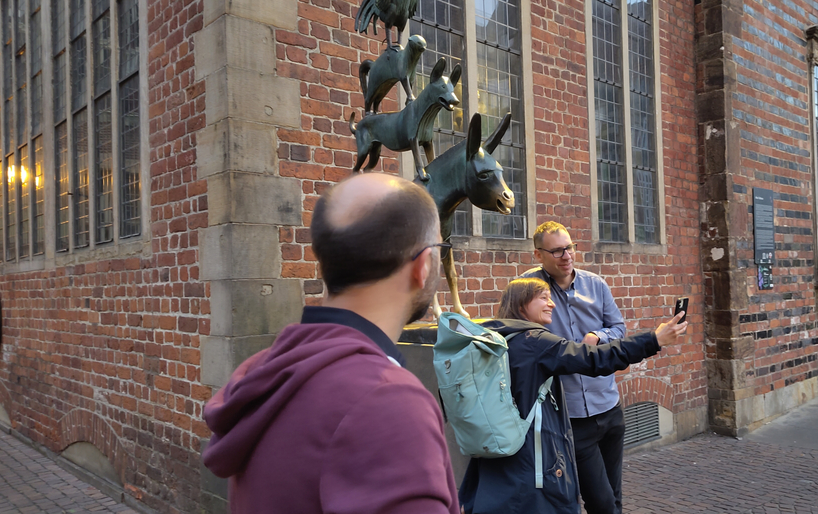
\includegraphics[width=.7\textwidth]{img/Bremen_Redaktionsorte.jpg}
\caption{Redaktionsorte XXVI: Bremen}
\end{figure}

Immerhin, um dem Ganzen auch etwas Positives abzugewinnen: Die
eingereichten und in die Ausgabe publizierten Beiträge haben offenbar
auf den Einsatz von Large Language Models (LLMs) als
\enquote{Betrugsmaschinen} verzichtet. Stattdessen setzen sie sich damit
auseinander, welchen Einfluss betrügerische Praxen im
Wissenschaftssystem haben und wie die Aufmerksamkeit dafür erhöht werden
kann. Auch wir haben keine gefälschten Artikel erstellt, um zu zeigen,
dass es geht. Es scheint nicht, als wäre Lug und Trug im
Bibliothekswesen (bei uns oder auch bei den anderen Zeitschriften in
unserem Bereich) ein relevantes Problem. In einer Welt, die aus Krisen
und Problemen zu bestehen scheint, mag diese moralische Integrität als
Pluspunkt gelten.

Mit Wünschen und Hoffnungen auf bessere Zeiten

Ihre/Eure Redaktion LIBREAS

(Berlin, Brandenburg an der Havel, Chur, Göttingen, München)

%autor

\end{document}